% ============================================================
%  מחוברים תמיד: טכנולוגיה וחיי היומיום
%  הקובץ הראשי. הידור:  xelatex main → biber main → xelatex main ×2
% ============================================================
\documentclass[11pt, a4paper, openany]{report}
\usepackage{style}
\addbibresource{refs.bib}

\begin{document}

% ---------- שער ----------
% ---------- עמוד שער ----------
\begin{titlepage}
\begin{tikzpicture}[remember picture, overlay]
  % רקע כחול-לילה
  \fill[night] (current page.south west) rectangle (current page.north east);
  % איור הרשת (נוצר ב-Python)
  \node[anchor=center, opacity=0.95] at ($(current page.center)+(0,1.2)$)
       {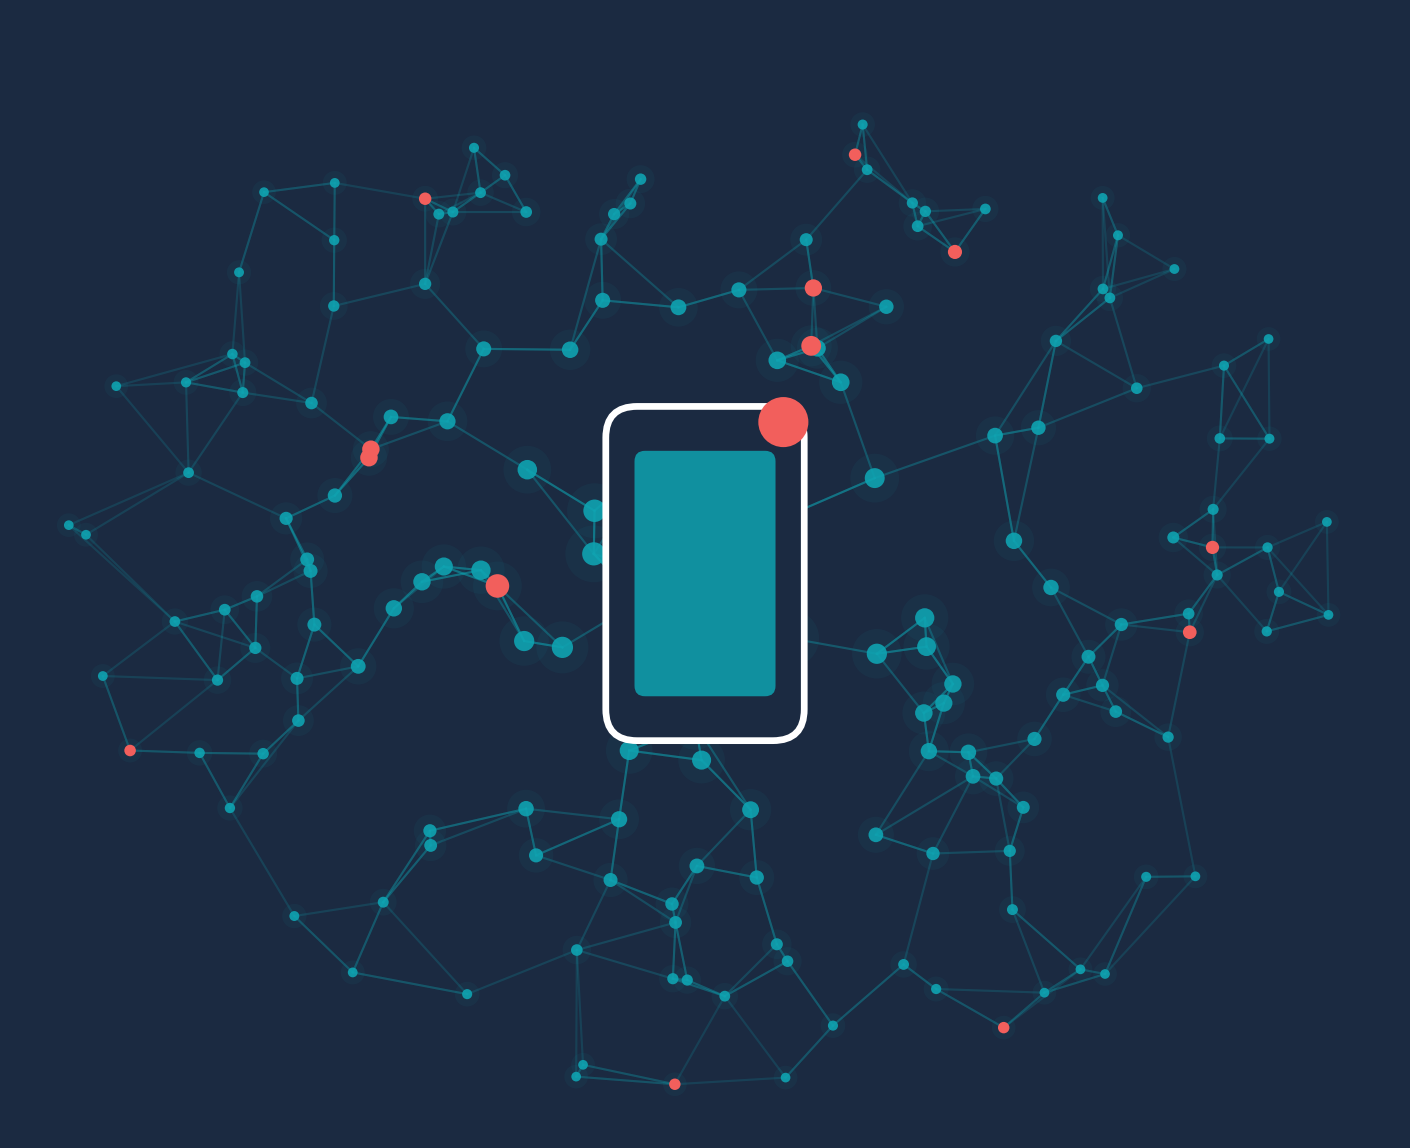
\includegraphics[width=\paperwidth]{images/cover_network.png}};
  % פס טורקיז
  \fill[screen] ($(current page.south west)+(0,4.2)$) rectangle ($(current page.south east)+(0,4.45)$);
  % כותרת
  \node[text=white, font=\headfont\bfseries\fontsize{48}{52}\selectfont, align=center]
       at ($(current page.north)+(0,-4.2)$) {\RL{מחוברים תמיד}};
  \node[text=screen, font=\headfont\fontsize{20}{24}\selectfont, align=center]
       at ($(current page.north)+(0,-5.7)$) {\RL{טכנולוגיה וחיי היומיום}};
  % נקודת התראה
  \fill[notif] ($(current page.north)+(5.6,-3.0)$) circle (0.35);
  \node[text=white, font=\headfont\bfseries\small] at ($(current page.north)+(5.6,-3.0)$) {\LR{9}};
  % פרטים בתחתית
  \node[text=white, font=\headfont\large, align=center]
       at ($(current page.south)+(0,2.9)$) {\RL{ספר שנכתב ב-\LR{LaTeX} בעזרת צוות סוכני בינה מלאכותית}};
  \node[text=white!70, font=\headfont, align=center]
       at ($(current page.south)+(0,2.0)$) {\RL{שנהב סולימאן \quad|\quad 2026}};
\end{tikzpicture}
\end{titlepage}


% ---------- תקציר ותוכן עניינים ----------
\pagenumbering{roman}
\chapter*{תקציר}
\addcontentsline{toc}{chapter}{תקציר}
\markboth{תקציר}{}

לפני מאתיים שנה, מידע נע במהירות של סוס. היום הוא נע במהירות האור, והוא כמעט אף פעם לא נח. הספר הזה שואל שאלה פשוטה לכאורה: מה קורה לבני אדם כשהם מחוברים תמיד?

כדי לענות עליה, הספר מתחיל רחוק מאוד מהמסך. הוא חוזר אל המברק של המאה ה-19, עובר דרך הרשת הצבאית שהפכה לאינטרנט, ומגיע אל המכשיר הקטן שבכיס, זה שבלע את המצלמה, המפה, הדואר והטלוויזיה. משם הוא עובר לנתונים: כ-5.87 מיליארד בני אדם השתמשו באינטרנט ב-2024 \parencite{itu2026data}, ומשתמש טיפוסי מבלה ברשת כ-6 שעות ו-40 דקות ביום \parencite{kemp2024}.

בהמשך, הספר בוחן את \textbf{כלכלת הקשב}, המנגנון שהופך כל גלילה לסחורה; את הקשר המורכב בין זמן מסך לרווחה נפשית, בעזרת מודל גולדילוקס פשוט, להמחשה בלבד, שמזמין לשאול לא רק "כמה מסך" אלא "כמה מכל דבר", ומזכיר שהאפקט שנמדד בפועל קטן; ואת הבית החכם, שבו הנוחות והפרטיות מושכות לכיוונים מנוגדים. הספר נחתם בארגז כלים מעשי לאיזון דיגיטלי ובמבט אל עידן הבינה המלאכותית.

אין כאן קריאה לזרוק את הטלפון לים. יש כאן הזמנה לעצור לרגע, להרים את הראש מהמסך, ולשאול מי בעצם מחזיק במי.

\keywords{זמן מסך, כלכלת הקשב, רווחה נפשית, השערת גולדילוקס, האינטרנט של הדברים, איזון דיגיטלי, \mbox{\en{Digital Well-being}}}

{\hypersetup{linkcolor=night}\tableofcontents}
\clearpage
\pagenumbering{arabic}

% ---------- פרקים ----------
\chapter{מבוא: יום אחד בחיים מחוברים}

\begin{epigraph}{}
פעם שאלנו "מה השעה?". היום אנחנו שואלים "כמה סוללה נשארה?". אולי זו השאלה החשובה יותר.
\end{epigraph}

\section{שבע בבוקר, בכל מקום בעולם}

השעון המעורר מצלצל. היד נשלחת אל השידה עוד לפני שהעיניים נפתחות. היא לא מחפשת משקפיים, לא כוס מים ולא את בן הזוג. היא מחפשת את הטלפון.

בתוך שלושים שניות כבר ידוע לכם מה מזג האוויר, מי כתב לכם בלילה, מה קרה בצד השני של כדור הארץ, ואיזה חבר מהתיכון נסע לתאילנד. עוד לא קמתם מהמיטה, ומאות בני אדם כבר נכנסו לחדר השינה שלכם.

הסצנה הזאת חוזרת על עצמה מיליארדי פעמים בכל בוקר. בתל אביב, בלאגוס ובסאו פאולו. אצל סטודנטית בירושלים ואצל נהג מונית בג'קרטה. לפי ההערכה המעודכנת של איגוד התקשורת הבין-לאומי, כ-5.87 מיליארד בני אדם השתמשו באינטרנט ב-2024, כ-\num{72.3\%} מאוכלוסיית העולם \parencite{itu2026data}. מעולם לא היה דבר כל כך משותף לכל כך הרבה בני אדם. לא דת, לא שפה ולא מטבע.

ובכל זאת, כדאי לזכור גם את הצד השני של המספר. אם כ-\num{72\%} מהאנושות מחוברים, פירוש הדבר שכ-\num{28\%} עדיין אינם מחוברים \parencite{itu2026data}. מיליארדי בני אדם חיים בעולם שבו "לבדוק בגוגל" איננו פועל יומיומי. הם לא מתגעגעים לרשת, כי מעולם לא חיו בתוכה. אבל העולם שסביבם, הבנקים, בתי הספר ומשרדי הממשלה, עובר אליה במהירות. הניתוק, שפעם היה מצב טבעי, הופך בהדרגה לסוג חדש של עוני.

וישראל? בתחילת 2025 כ-\num{91.1\%} מהישראלים היו מחוברים לרשת \parencite{kemp2025israel}. במדינה שבה קשה להסכים כמעט על כל דבר, הסמארטפון הוא אולי הקונצנזוס האחרון.

\section{המהפכה השקטה}

מהפכות גדולות נוטות להיות רועשות. למהפכה החקלאית נדרשו אלפי שנים, והיא שינתה את גוף האדם, את המשפחה ואת הנוף. המהפכה התעשייתית מילאה את השמיים בעשן. המהפכה הדיגיטלית, לעומתן, נכנסה לחיינו בשקט כמעט מוחלט. היא לא שרפה ערים ולא הפילה מלכים. היא רק ביקשה מאיתנו ללחוץ על "אני מסכים".

והיא לא נשארה בכיס. לפי הדוח הגלובלי של \en{DataReportal}, משתמש אינטרנט טיפוסי מבלה ברשת חלק ניכר מכל יום \parencite{kemp2024}. חשבון פשוט ממחיש עד כמה.

\begin{factbox}[נתון מפתח]
\textbf{6 שעות ו-40 דקות} ביום ברשת, אצל משתמש אינטרנט טיפוסי \parencite{kemp2024}. אם תכפילו את זה ב-365 ימים, תקבלו כ-2,430 שעות בשנה, קצת יותר ממאה ימים שלמים. במילים אחרות, וזה כבר החשבון שלנו ולא של הדוח: משתמש כזה מבלה בכל שנה יותר משלושה חודשים "בתוך" המסך.
\end{factbox}

אבל המספרים לבדם לא מספרים את הסיפור. השאלה המעניינת איננה כמה זמן אנחנו מבלים מול המסך, אלא מה המסך עושה לנו בזמן הזה. האם הוא כלי, כמו פטיש? או סביבה, כמו עיר? או אולי, וזו האפשרות המטרידה ביותר, הוא סוכן בעל אינטרסים משלו?

דמיינו ציידת-לקטת, הרבה לפני הכתב. כדי לשרוד, היא הייתה צריכה להכיר את הצמחים סביבה ואת עקבות בעלי החיים. הידע שלה, מן הסתם, היה בראש. אנחנו מחזיקים בכיס גישה לכמעט כל הידע האנושי, אבל לא תמיד זוכרים את מספר הטלפון של אמא. זה לא בהכרח רע. זה פשוט שונה. וכדאי להבין את השינוי לפני שמחליטים אם הוא טוב.

יש עוד הבדל, עדין יותר. בלי כתב ובלי דואר, אפשר היה להכיר לעומק רק את מי שחי בסביבה הקרובה. אנחנו מחוברים למאות ולאלפים, אבל רובם מוכרים לנו רק כתמונה קטנה ועיגול ירוק שמסמן "מחובר עכשיו". זו השערה ולא ממצא, אבל קשה להשתחרר ממנה: אם המוח שלנו עוצב בעולם של קהילות קטנות, הוא נדרש היום לעקוב אחרי כפר גלובלי שלם. לא פלא אם לפעמים הוא מתעייף.

\begin{thinkbox}
נסו להיזכר: מתי בפעם האחרונה עברה עליכם שעה שלמה, בהכרה מלאה, בלי לגעת במסך כלשהו? אם קשה לכם להיזכר, שאלו את עצמכם: האם זו הייתה בחירה שלכם?
\end{thinkbox}

\section{מה הספר הזה מנסה לעשות}

הספר הזה לא נכתב כדי להפחיד, וגם לא כדי לחגוג. הוא מנסה לעשות משהו צנוע יותר וקשה יותר: להסתכל על הטכנולוגיה של חיי היומיום מגובה רב, כמו שהיסטוריון מסתכל על אימפריה, ובאותו זמן מקרוב מאוד, כמו שמסתכלים על המסך בשתיים בלילה.

המסע שלפניכם בנוי משבעה פרקים נוספים:

\begin{enumerate}
  \item \textbf{מהטלגרף לסמארטפון}: איך הגענו לכאן, ולמה כל המצאה חדשה בתקשורת נראתה לבני דורה כסוף העולם.
  \item \textbf{אנטומיה של יום דיגיטלי}: לאן באמת הולכות השעות, ולמה בדרום אפריקה מבלים ברשת כמעט פי שניים מאשר בדנמרק.
  \item \textbf{כלכלת הקשב}: מי מרוויח מהגלילה שלכם, ואיך זה עובד.
  \item \textbf{זמן מסך ורווחה}: מה המדע יודע, ובעיקר מה הוא עדיין לא יודע.
  \item \textbf{הבית החכם}: כשהמקרר, הנורה והשואב מתחילים לדבר ביניהם.
  \item \textbf{איזון דיגיטלי}: ארגז כלים מעשי, בלי מוסר ובלי אשמה.
  \item \textbf{סיכום ומבט לעתיד}: מה קורה כשהמכונה מתחילה לדבר בחזרה.
\end{enumerate}

לאורך הדרך תמצאו תיבות צבעוניות: נתוני מפתח, אזהרות, טיפים ושאלות למחשבה. את רוב השאלות לא נפתור. אבל לפעמים שאלה טובה שווה יותר מתשובה מהירה. בעיקר בעידן שבו תשובות מהירות נמצאות במרחק הקלקה אחת.

\chapter{מהטלגרף לסמארטפון}

\begin{epigraph}{}
כל דור בטוח שהוא הראשון שהטכנולוגיה מבלבלת. כל דור טועה, וכל דור צודק.
\end{epigraph}

\section{הודעה שנעה במהירות של רגליים}

במשך רוב ההיסטוריה האנושית, מהירות המידע הייתה שווה למהירות הגוף. ציידת-לקטת שרצתה לספר לשבט השכן שנמצא מעיין חדש הייתה צריכה ללכת לשם. מלך שרצה לשלוח פקודה לגבול הממלכה שלח רץ, ואחר כך פרש. גם האימפריות הגדולות של העולם העתיק, עם הדרכים הסלולות ותחנות הדואר שלהן, לא הצליחו לשבור את החוק הבסיסי הזה: הודעה לא יכולה לנוע מהר יותר מהשליח שנושא אותה.

הדפוס של המאה ה-15 שינה את \textbf{כמות} המידע, אבל לא את מהירותו. ספר מודפס עדיין נסע בעגלה. הידיעה על מותו של מלך יכלה להגיע לפינות הממלכה שבועות אחרי שהוכתר יורשו.

ואז, במאה ה-19, קרה משהו מוזר. המידע התנתק מהחומר.

\section{המברק: כשהמילים עזבו את הסוס}

ב-24 במאי 1844 שלח סמואל מורס את המברק הציבורי הראשון, מוושינגטון לבולטימור. ארבע מילים מהתנ"ך, \en{"What hath God wrought"}, עברו בין שתי הערים כמעט ברגע. לראשונה בהיסטוריה, הודעה הגיעה לפני השליח. למעשה, לא היה שליח בכלל.

קל לזלזל בזה היום, כשהודעת \en{WhatsApp} מגיעה לאוסטרליה בפחות משנייה. אבל עבור בני הדור ההוא זה היה דבר מדהים. עיתונים התחילו לפרסם חדשות מערים רחוקות מאתמול, ולא מהחודש שעבר. בורסות בערים שונות התחילו לנשום באותו קצב. והפילוסופים של התקופה כבר דאגו: האם האנושות מסוגלת לעכל כל כך הרבה מידע, כל כך מהר?

שימו לב לשאלה הזאת. היא תחזור בכל פרק בספר.

\section{מרשת צבאית לרשת עולמית}

בעשורים שאחרי המברק הגיעו הטלפון, הרדיו והטלוויזיה. כל אחד מהם הוסיף משהו: את הקול, את ההמונים, את התמונה. אבל כולם עבדו לפי אותו היגיון: ערוץ אחד, מסר אחד, וקהל שמקבל.

השינוי האמיתי התחיל במעבדות. בסוף אוקטובר 1969 נשלחה ההודעה הראשונה ברשת \en{ARPANET}, מאוניברסיטת \en{UCLA} אל מחשב מרוחק. זו הייתה רשת של חוקרים ושל משרד ההגנה האמריקאי, לא של אזרחים. כמעט אף אחד לא שם לב.

ב-1989 הגיש טים ברנרס-לי, מהנדס תוכנה במעבדת \en{CERN}, מסמך פנימי בשם "ניהול מידע: הצעה" \parencite{berners1989}. הבוס שלו רשם עליו, לפי המסורת, שההצעה "מעורפלת, אבל מרגשת". מן ההצעה המעורפלת הזאת נולד ה-\en{World Wide Web}. האינטרנט הפסיק להיות רשת של מומחים והתחיל להפוך לעיר שבה כולם יכולים לגור.

\begin{thinkbox}
המברק, הטלפון והאינטרנט נולדו כולם מתוך צורך מעשי: עסקים, צבא, מדע. אף אחד מהממציאים לא תכנן לשנות את הדרך שבה מתבגרים מתאהבים או מתווכחים. האם ייתכן שההשפעות החשובות ביותר של טכנולוגיה הן תמיד אלה שאיש לא תכנן?
\end{thinkbox}

\section{המכשיר שבלע את העולם}

ב-9 בינואר 2007 עלה סטיב ג'ובס לבמה והציג את ה-\en{iPhone}. בהודעה לעיתונות תיארה אותו אפל כשלושה מוצרים במכשיר אחד: טלפון נייד, נגן מוזיקה עם מסך מגע, ומכשיר לתקשורת באינטרנט \parencite{apple2007}. בדיעבד, זו הייתה הערכה צנועה מאוד. הסמארטפון בלע גם את המצלמה, המפה, השעון, הפנס, הארנק, הספרייה והטלוויזיה. הוא הפך לשלט הרחוק של החיים כולם.

ואז הגיעו הרשתות החברתיות, שצמחו בשנות ה-2000 וה-2010, והפכו את המכשיר מכלי לקבלת מידע לבמה שעליה כל אחד משדר. ולבסוף, ב-30 בנובמבר 2022, השיקה \en{OpenAI} את \en{ChatGPT} כ"תצוגה מקדימה למחקר" \parencite{openai2022}. לראשונה, המכונה לא רק העבירה את המילים שלנו. היא התחילה לכתוב משלה.

טבלה~\ref{tab:timeline} מסכמת את אבני הדרך העיקריות במסע הזה.

\begin{table}[htbp]
\centering
\caption{ציר זמן: מהמברק לבינה המלאכותית}
\label{tab:timeline}
\begin{tabularx}{\textwidth}{@{}>{\centering\arraybackslash}p{3.9cm} l X@{}}
\toprule
\textbf{שנה} & \textbf{המצאה} & \textbf{מה השתנה} \\
\midrule
1844 & המברק של מורס & המידע נע מהר יותר מהשליח \\
סוף המאה ה-19 & הטלפון & הקול האנושי חוצה מרחקים \\
שנות ה-20 של המאה ה-20 & הרדיו & תקשורת המונים בזמן אמת \\
אמצע המאה ה-20 & הטלוויזיה & התמונה נכנסת לסלון \\
1969 & \en{ARPANET} & מחשבים מתחילים לדבר זה עם זה \\
1973 & הטלפון הנייד & שיחה בלי חוטים, מהרחוב \\
1989 & הצעת ה-\en{Web} ב-\en{CERN} & רשת שכל אחד יכול לגלוש בה \parencite{berners1989} \\
שנות ה-2000 וה-2010 & הרשתות החברתיות & כל אדם הופך לתחנת שידור \\
2007 & ה-\en{iPhone} & האינטרנט עובר לכיס \parencite{apple2007} \\
2022 & \en{ChatGPT} & המכונה מתחילה לכתוב ולשוחח \parencite{openai2022} \\
\bottomrule
\end{tabularx}
\end{table}

\section{כמעט שישה מיליארד}

\begin{sloppypar}
איור~\ref{fig:internet-users} מראה את קצב ההתפשטות. ב-2005 השתמשו באינטרנט כמיליארד בני אדם, כ-15.7\% מאוכלוסיית העולם. ב-2015 היו אלה כ-2.96 מיליארד, וב-2024 כבר כ-5.87 מיליארד, כ-72.3\% מהאנושות \parencite{itu2026data}. בתוך פחות מעשרים שנה, מספר המחוברים גדל כמעט פי שישה.
\end{sloppypar}

% גרף Python: python/make_graphs.py → images/internet_users.png
\begin{figure}[htbp]
\centering
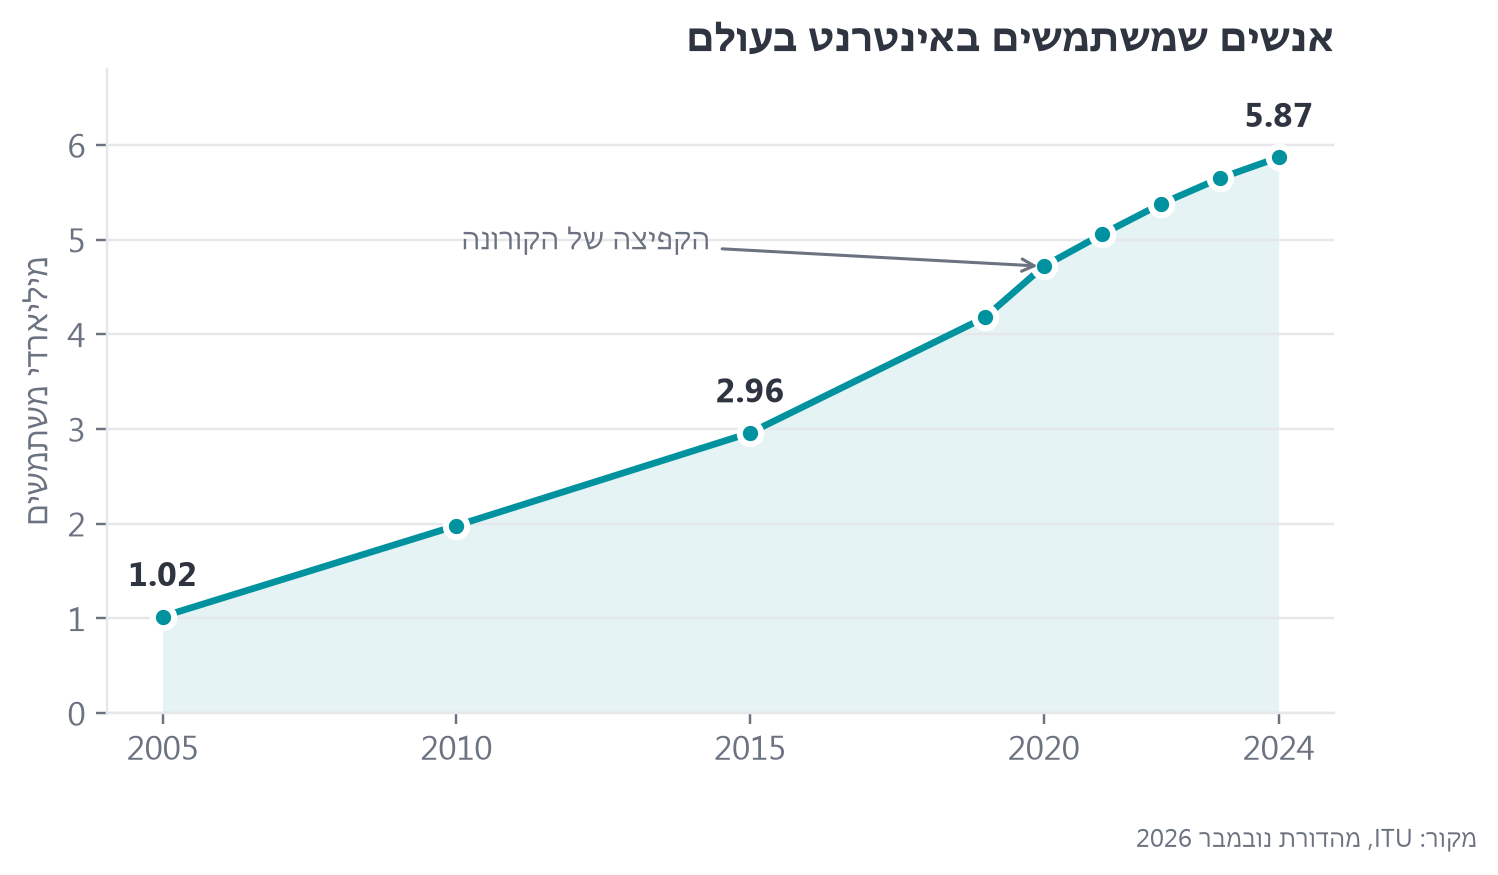
\includegraphics[width=0.92\textwidth]{images/internet_users.png}
\caption{מספר משתמשי האינטרנט בעולם, במיליארדים, 2005--2024 \parencite{itu2026data}. הגרף נוצר ב-\en{Python}.}
\label{fig:internet-users}
\end{figure}


שימו לב לקפיצה שבין 2019 ל-2020: מ-4.18 ל-4.72 מיליארד \parencite{itu2026data}. הנתונים עצמם אינם אומרים מה גרם לקפיצה. ההסבר שמתבקש, וזו פרשנות שלנו ולא ממצא של המקור, הוא מגפת הקורונה, שדחפה אנשים רבים אל המסך, ללימודים, לעבודה ולשיחות עם סבתא. אם זה אכן ההסבר, משבר עולמי אחד עשה בשנה מה שבדרך כלל לוקח כמה שנים.

\begin{factbox}[מספרים שזזים]
גם המספרים עצמם אינם יציבים. במהדורת 2024 של \en{Facts and Figures} העריך איגוד התקשורת הבין-לאומי שבשנה זו היו מחוברים כ-5.5 מיליארד בני אדם \parencite{itu2024}, ואילו בסדרה המעודכנת ההערכה לאותה שנה היא כ-5.87 מיליארד \parencite{itu2026data}. ההבדל נובע מתיקוני מתודולוגיה. בספר הזה אנחנו משתמשים בסדרה המעודכנת בלבד, כדי שהגרף והטקסט ידברו באותה שפה.
\end{factbox}

מהסוס ועד הסמארטפון עברו פחות מ-200 שנה. זה הרף עין במונחים של ההיסטוריה האנושית. הגוף שלנו, המוח שלנו והרגלי השינה שלנו עוצבו במשך מאות אלפי שנים בעולם שבו המידע הגיע לאט. עכשיו הוא מגיע בלי הפסקה. בפרק הבא ננסה להבין מה זה עושה ליום אחד בחיים שלנו.

\chapter{אנטומיה של יום דיגיטלי}

\begin{epigraph}{}
אנחנו לא מבזבזים זמן על המסך. אנחנו משלמים בו. השאלה היא רק מה אנחנו מקבלים בתמורה.
\end{epigraph}

\section{6 שעות ו-40 דקות}

לאיכר בימי הביניים היה יום ברור. הוא קם עם השמש, עבד בשדה, אכל, התפלל וישן כשהחשיך. השמש הייתה השעון, העונות היו לוח השנה, והכנסייה הייתה ערוץ החדשות היחיד.

היום שלנו בנוי אחרת. הוא מחולק לא לפי השמש אלא לפי המסכים. לפי הדוח הגלובלי \en{Digital 2024}, משתמש אינטרנט טיפוסי מבלה ברשת כ-6 שעות ו-40 דקות ביום, כ-400 דקות \parencite{kemp2024}. שנה קודם לכן היה המספר 6 שעות ו-36 דקות. כלומר, אחרי שנים של זינוק, הוא כמעט התייצב. אולי הגענו לתקרה. אולי פשוט נגמרו לנו השעות.

כדי להבין את המספר הזה, כדאי לחשוב עליו כעל תקציב. אם אתם ישנים כשמונה שעות, נשארות לכם כשש-עשרה שעות שבהן אתם ערים. מתוכן, כ-\num{40\%} עוברות ברשת. ולא מדובר רק בגלילה בטלפון: גם העבודה מול המחשב, הסדרה בערב והניווט ברכב נכנסים לחשבון. הרשת היא כבר לא מקום שהולכים אליו. היא המקום שבו אנחנו נמצאים.

\section{לאן הולך הזמן}

טבלה~\ref{tab:daily-time} מפרקת את התקציב היומי לכמה מרכיבים מרכזיים, לפי הנתונים שפורסמו בדוח.

\begin{table}[htbp]
\centering
\caption{זמן יומי ממוצע לפי פעילות (משתמש טיפוסי, 2024)}
\label{tab:daily-time}
\begin{tabularx}{0.9\textwidth}{@{}X c@{}}
\toprule
\textbf{פעילות} & \textbf{זמן ליום (שעות:דקות)} \\
\midrule
סך כל הזמן ברשת & \num{6:40} \\
רשתות חברתיות & \num{2:23} \\
טלוויזיה משודרת (ליניארית) & \num{1:44} \\
טלוויזיה בכל הפורמטים, כולל סטרימינג & \num{>3:00}\textsuperscript{*} \\
\bottomrule
\end{tabularx}

\vspace{0.3em}
{\small\sffamily מקור: \textcite{kemp2024}. הפעילויות חופפות זו לזו, ולכן אינן מסתכמות לסך הכולל. \textsuperscript{*}הדוח מוסר רק שהזמן עולה על שלוש שעות, בלי ערך מדויק.}
\end{table}

הרשתות החברתיות לבדן לוקחות כ-2 שעות ו-23 דקות ביום \parencite{kemp2024}. נסו להשוות את זה לזמן שאתם מקדישים לארוחות, לספורט ולשיחה פנים אל פנים עם בני המשפחה, ביחד. המעניין הוא שהמספר הזה דווקא ירד מעט, מ-2 שעות ו-31 דקות בשנה הקודמת, אבל לפי הדוח עצמו, רוב הירידה נובעת משינוי בשיטת המדידה \parencite{kemp2024}. גם לסטטיסטיקה יש מצבי רוח.

והטלוויזיה? הקופסה שהייתה פעם מרכז הסלון לא מתה. היא רק שינתה צורה. הצפייה בטלוויזיה המשודרת ירדה לשעה ו-44 דקות ביום, לעומת שעה ו-58 דקות ב-2019, אבל כשמחברים את כל הפורמטים, כולל סטרימינג, מגיעים ליותר משלוש שעות ביום \parencite{kemp2024}. הטלוויזיה לא נעלמה. היא נכנסה לטלפון.

\begin{alertbox}[למה הטבלה לא "מסתכמת"]
אפשר לצפות בסדרה תוך כדי גלילה בטלפון, ולשמוע פודקאסט בזמן שעונים להודעות. לכן אסור לחבר את השורות בטבלה ולצפות לקבל את הסך הכולל. אנחנו לא רק מבלים זמן רב מול מסכים. לעיתים קרובות אנחנו מבלים אותו מול כמה מסכים בבת אחת.
\end{alertbox}

\section{מפת העולם של זמן המסך}

ממוצע עולמי מסתיר הבדלים עצומים. איור~\ref{fig:daily-time} משווה בין כמה מדינות. בדרום אפריקה משתמש טיפוסי מבלה ברשת כ-9 שעות ו-24 דקות ביום. בברזיל כ-9 שעות ו-13 דקות, ובפיליפינים כ-8 שעות ו-52 דקות. בקצה השני נמצאות דרום קוריאה, עם כ-5 שעות ו-19 דקות, ודנמרק, עם כ-5 שעות ו-8 דקות \parencite{kemp2024}. ביפן הממוצע נמוך עוד יותר, פחות מארבע שעות ביום \parencite{kemp2024}.

% גרף Python: python/make_graphs.py → images/daily_time.png
\begin{figure}[htbp]
\centering
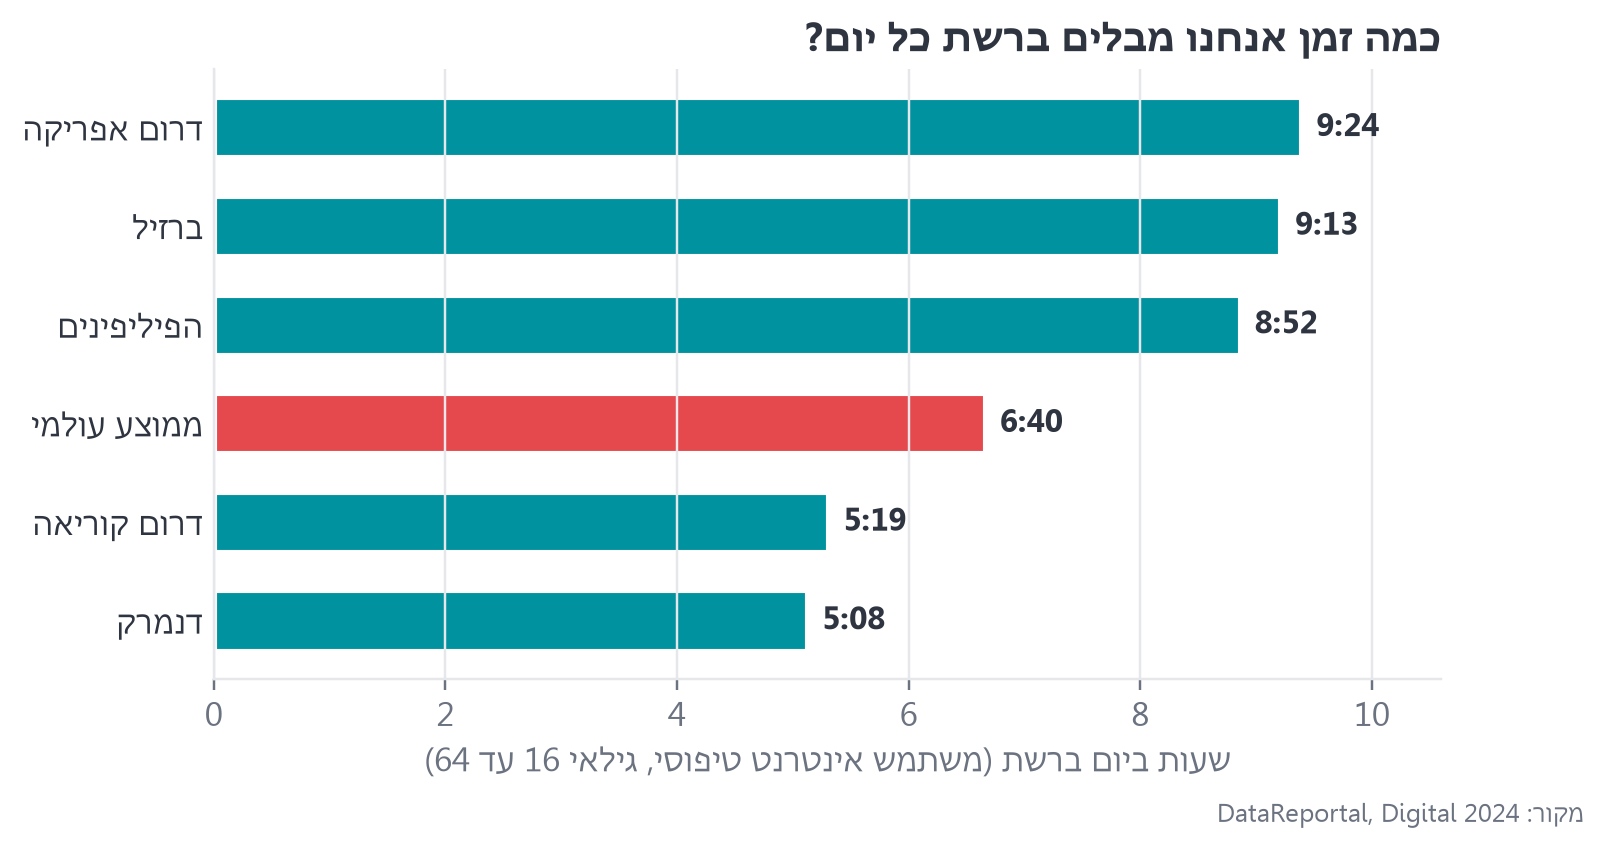
\includegraphics[width=0.92\textwidth]{images/daily_time.png}
\caption[זמן יומי ממוצע ברשת לפי מדינה]{זמן יומי ממוצע ברשת במדינות נבחרות לעומת הממוצע העולמי \parencite{kemp2024}. הגרף נוצר ב-\en{Python}.}
\label{fig:daily-time}
\end{figure}


איך מסבירים את הפער? אפשר היה לנחש שהמדינות העשירות והטכנולוגיות ביותר יובילו. אבל דרום קוריאה, אחת המדינות המחוברות והמתקדמות בעולם, נמצאת דווקא סמוך לתחתית האיור. חשוב לזכור שאת המדינות באיור בחרנו אנחנו, מתוך אלה שהדוח מזכיר בטקסט, כדי להמחיש את הטווח. זו לא רשימה מלאה ולא דירוג. הנתונים לבדם לא מסבירים את הסיבה, וכדאי להיזהר מתשובות מהירות. ייתכן שיש לכך קשר לשעות העבודה, לגיל האוכלוסייה, למזג האוויר או לתרבות של בילוי מחוץ לבית. ייתכן שבמקומות שבהם הטלפון הוא המחשב היחיד, הוא גם הקולנוע, הבנק והכיכר העירונית. הדבר הבטוח היחיד הוא שזמן מסך איננו גזירת גורל טכנולוגית. הוא גם עניין של תרבות.

\begin{factbox}[קנה המידה]
בתחילת \num{2024} היו בעולם כ-\num{5.35} מיליארד משתמשי אינטרנט וכ-\num{5.04} מיליארד "זהויות" ברשתות חברתיות \parencite{kemp2024}. המספר נמוך מ-\num{5.87} המיליארד שבפרק הקודם, כי מדובר במקור אחר: \en{DataReportal} מודד את תחילת השנה ובשיטה משלו, ואילו \en{ITU} מעריך את השנה כולה, ובסדרה המעודכנת. זהויות, לא אנשים: לאדם אחד יכולים להיות כמה חשבונות, ולחשבון אחד יכולים להיות כמה בעלים.
\end{factbox}

\section{הזמן כמטבע}

לכל ציוויליזציה היה מטבע משלה. מלח, צדפים, זהב, שטרות. בעולם הדיגיטלי מתגבש מטבע חדש: \textbf{הזמן שלכם}. כשאפליקציה מציעה לכם שירות "בחינם", היא לא באמת מוותרת על תשלום. היא פשוט גובה אותו בדקות.

הכלכלנים מדברים על "עלות אלטרנטיבית": המחיר האמיתי של כל דבר הוא מה שוויתרנו עליו כדי להשיג אותו. עלות אלטרנטיבית של שעה בגלילה היא שעה של שינה, ספר, ריצה או שיחה. זה לא אומר שהגלילה תמיד גרועה. לפעמים היא בדיוק מה שצריך אחרי יום ארוך. אבל זה אומר שכדאי לפחות לדעת שמשלמים.

וזה מעלה שאלה מטרידה. אם 400 דקות ביום הן תקציב, מי מחליט איך להוציא אותו? האם אתם קובעים מתי לפתוח את האפליקציה, או שהאפליקציה קובעת מתי לקרוא לכם? בפרק הבא נגלה שמאחורי השאלה הזאת עומדת תעשייה שלמה, ושיש לה תשובה ברורה מאוד.

\begin{thinkbox}
אם הייתם צריכים לשלם שקל אחד על כל דקה ברשתות החברתיות, כמה הייתם מוציאים החודש? ועל אילו דקות הייתם מוותרים ראשונות?
\end{thinkbox}

\chapter{כלכלת הקשב}
\label{ch:attention}

\begin{epigraph}{הרברט סיימון, 1971}
מה שמידע צורך הוא די ברור: הוא צורך את תשומת הלב של מקבליו.
\end{epigraph}

\section{עוני של קשב}

במשך רוב ההיסטוריה, מידע היה משאב נדיר. ספר היה אוצר. מכתב היה אירוע. מי ששלט במידע, הכוהנים, הסופרים והשליטים, שלט בחברה. הבעיה של בני האדם הייתה תמיד מחסור במידע.

ב-1971, הרבה לפני הסמארטפון ואפילו לפני המחשב האישי, הבחין הכלכלן והמדען הרברט סיימון שהמשוואה עומדת להתהפך. מידע, כתב סיימון, איננו בחינם. הוא צורך משהו: את תשומת הלב של מי שקולט אותו. ומכאן המסקנה שלו, שנשמעת היום כמו נבואה: \textbf{שפע של מידע יוצר עוני של קשב} \parencite{simon1971}.

חשבו על זה רגע. היום יש בכיס שלכם יותר מידע מאשר בכל הספריות של העולם העתיק גם יחד. אבל יש לכם בדיוק אותן 24 שעות ביממה שהיו לאריסטו. המידע הפך לזול כמו מים. הקשב נשאר יקר כמו זהב. וכשמשהו נדיר ויקר, מישהו תמיד ימצא דרך לסחור בו.

\section{סוחרי הקשב}

הרעיון למכור קשב לא נולד בעמק הסיליקון. טים וו, משפטן והיסטוריון של התקשורת, מתאר בספרו "סוחרי הקשב" כיצד העיקרון התגבש כבר במאה ה-19, עם עיתוני הפרוטה הזולים, ועבר משם לרדיו, לטלוויזיה ולבסוף לרשתות החברתיות \parencite{wu2016}. המודל העסקי פשוט: נותנים לקהל תוכן בחינם או כמעט בחינם, אוספים את תשומת הלב שלו, ומוכרים אותה למפרסמים.

ההבדל בין עיתון הפרוטה לבין הפיד שלכם איננו בעיקרון אלא בדיוק. העיתון ידע בערך מי קורא אותו. האפליקציה יודעת בדיוק כמה שניות התעכבתם על כל תמונה.

ויש הבדל נוסף. עיתון נגמר. בעמוד האחרון יש תשבץ, ואחריו אין כלום. גם שידורי הטלוויזיה היו נגמרים פעם בחצות, עם המנון ופס צבעים. הפיד, לעומת זאת, איננו נגמר לעולם. אין לו עמוד אחרון, ולכן ההחלטה מתי להפסיק עוברת כולה אלינו, בדיוק בשעה שבה אנחנו הכי עייפים.

\begin{factbox}[המשפט שכדאי לזכור]
אם אינכם משלמים על המוצר, סביר להניח שאתם לא הלקוחות. אתם חומר הגלם. הלקוחות הם המפרסמים, והמוצר הוא הקשב שלכם.
\end{factbox}

\section{מודל ה-\texorpdfstring{\en{Hook}}{Hook}}

איך גורמים לאדם לחזור לאפליקציה עשרות פעמים ביום, בלי שאיש מכריח אותו? ניר אייל, יועץ ומחבר הספר \en{Hooked}, תיאר ב-2014 מודל לבניית מוצרים שיוצרים הרגל \parencite{eyal2014}. המודל בנוי מארבעה שלבים שחוזרים על עצמם במעגל: \textbf{טריגר}, \textbf{פעולה}, \textbf{תגמול משתנה} ו\textbf{השקעה}.

הלב של המודל הוא התגמול ה\textbf{משתנה}. אילו כל פתיחה של האפליקציה הייתה מניבה בדיוק אותו דבר, היינו משתעממים מהר. אבל כשאיננו יודעים מה מחכה לנו, לייק, הודעה מאדם שאנחנו אוהבים או סתם כלום, אנחנו חוזרים שוב ושוב. מכונות המזל בקזינו עובדות על אותו עיקרון בדיוק. ההבדל הוא שאת מכונת המזל הזאת אנחנו נושאים בכיס, והיא פתוחה עשרים וארבע שעות ביממה.

\section{מעגל בן שמונה שלבים}

מודל ה-\en{Hook} מסביר מה קורה בצד של המשתמש. אבל כדי להבין את כלכלת הקשב, צריך לראות גם את הצד השני של המסך. איור~\ref{fig:attention-loop} מחבר את שני הצדדים למעגל אחד בן שמונה שלבים.

% ---------- תרשים בלוקים: מעגל כלכלת הקשב (8 בלוקים) ----------
\begin{figure}[htbp]
\centering
\begin{tikzpicture}[
  blk/.style={rectangle, rounded corners=5pt, draw=#1, line width=1.2pt,
              fill=#1!12, text width=3.1cm, minimum height=1.25cm,
              align=center, font=\headfont\small, drop shadow={opacity=0.15}},
  blk/.default=screen,
  arr/.style={-{Stealth[length=3mm]}, line width=1.4pt, draw=night!70},
  num/.style={circle, fill=#1, text=white, font=\headfont\bfseries\footnotesize,
              inner sep=1.5pt, minimum size=1.3em},
]
  % מרכז
  \node[circle, fill=night, text=white, minimum size=2.6cm, align=center,
        font=\headfont\bfseries, text width=1.8cm] (core) at (0,0) {\RL{הקשב}\\ \RL{שלך}};

  % 8 בלוקים במעגל (נקראים עם כיוון השעון, מלמעלה)
  % \RL{} שומר על סדר המילים העברי בתוך צמתי TikZ
  \def\rad{4.9}
  \node[blk=notif]  (b1) at (90:\rad)  {\RL{\textbf{טריגר}}\\ \RL{התראה, רטט, נקודה אדומה}};
  \node[blk=notif]  (b2) at (45:\rad)  {\RL{\textbf{פעולה}}\\ \RL{פתיחת האפליקציה}};
  \node[blk=sun]    (b3) at (0:\rad)   {\RL{\textbf{תגמול משתנה}}\\ \RL{לייק? הודעה? סרטון?}};
  \node[blk=sun]    (b4) at (-45:\rad) {\RL{\textbf{השקעה}}\\ \RL{פוסט, תגובה, עוקבים}};
  \node[blk=screen] (b5) at (-90:\rad) {\RL{\textbf{איסוף נתונים}}\\ \RL{כל גלילה נרשמת}};
  \node[blk=screen] (b6) at (-135:\rad){\RL{\textbf{אלגוריתם}}\\ \RL{חיזוי מה יחזיק אותך}};
  \node[blk=night]  (b7) at (180:\rad) {\RL{\textbf{פרסום ממוקד}}\\ \RL{הקשב נמכר למפרסם}};
  \node[blk=night]  (b8) at (135:\rad) {\RL{\textbf{הכנסות}}\\ \RL{מימון פיצ'רים ממכרים}};

  % חיצים במעגל
  \foreach \a/\b in {b1/b2, b2/b3, b3/b4, b4/b5, b5/b6, b6/b7, b7/b8, b8/b1}
    \draw[arr] (\a) to[bend left=12] (\b);
  % חיצים מהמרכז
  \foreach \b in {b1,b3,b5,b7}
    \draw[-{Stealth}, dashed, draw=screen, line width=0.8pt] (core) -- (\b);

  % מספרי שלבים
  \foreach \b/\n/\c in {b1/1/notif, b2/2/notif, b3/3/sun, b4/4/sun,
                        b5/5/screen, b6/6/screen, b7/7/night, b8/8/night}
    \node[num=\c] at (\b.north east) {\n};
\end{tikzpicture}
\caption{מעגל כלכלת הקשב: שמונה שלבים שהופכים דקה של סקרנות לשעה של גלילה (עיבוד על בסיס מודל ה-\en{Hook} של \textcite{eyal2014} ו-\textcite{zuboff2019}).}
\label{fig:attention-loop}
\end{figure}


נלך במעגל, שלב אחר שלב:

\begin{enumerate}
  \item \textbf{טריגר}: הטלפון רוטט, נקודה אדומה מופיעה על האייקון. משהו קורא לכם.
  \item \textbf{פעולה}: אתם פותחים את האפליקציה. זה לוקח שנייה, ולא דורש מחשבה.
  \item \textbf{תגמול משתנה}: אולי לייק, אולי הודעה, אולי סרטון מצחיק. אי-הוודאות היא שמחזיקה אתכם.
  \item \textbf{השקעה}: אתם מגיבים, מעלים תמונה, עוקבים אחרי מישהו. כל השקעה כזאת מגדילה את הסיכוי שתחזרו.
  \item \textbf{איסוף נתונים}: כל גלילה, כל עצירה וכל הקלקה נרשמות.
  \item \textbf{אלגוריתם}: המערכת לומדת מה מחזיק דווקא אתכם, ומתאימה את התוכן הבא.
  \item \textbf{פרסום ממוקד}: הקשב שלכם, יחד עם מה שנלמד עליכם, נמכר למפרסמים.
  \item \textbf{הכנסות}: הכסף מושקע בחזרה בפיתוח פיצ'רים שמחזיקים אתכם עוד יותר, והמעגל מתחיל מחדש עם טריגר חדש.
\end{enumerate}

ארבעת השלבים הראשונים קורים אצלכם, בתודעה. ארבעת האחרונים קורים בשרתים, הרחק מהעיניים. ומה שהופך את המעגל לחזק כל כך הוא שכל סיבוב משפר את הסיבוב הבא. ככל שאתם גוללים יותר, האלגוריתם מכיר אתכם טוב יותר, וככל שהוא מכיר אתכם טוב יותר, קשה יותר להפסיק לגלול.

\begin{alertbox}[לא קונספירציה, מודל עסקי]
אין כאן חדר חשוך שבו מישהו זומם נגדכם. יש כאן מערכת שמכוונת להגדיל מדד אחד: זמן ומעורבות. כשמערכת חזקה מאוד ממקסמת מדד אחד, היא עלולה לפגוע בכל מה שאיננו נמדד, כמו שינה, ריכוז או שיחה בארוחת ערב.
\end{alertbox}

\section{קפיטליזם המעקב}

הסוציולוגית שושנה זובוף לוקחת את הטיעון צעד אחד קדימה. בספרה "עידן קפיטליזם המעקב" היא טוענת שהשיטה הזאת תובעת לעצמה את החוויה האנושית כ\textbf{חומר גלם חינמי} \parencite{zuboff2019}. החוויות שלנו מתורגמות לנתוני התנהגות. חלק מהנתונים משמש לשיפור השירות, אבל העודף, מה שזובוף מכנה \en{behavioral surplus}, הופך ל"מוצרי ניבוי": תחזיות על מה שנעשה, נקנה ונרגיש בהמשך.

כאן מסתתרת הקפיצה ההיסטורית. המהפכה התעשייתית הפכה את הטבע לחומר גלם: יערות, פחם, נפט. קפיטליזם המעקב, לפי זובוף, הופך את \textbf{הטבע האנושי} לחומר גלם. לא את מה שאנחנו מייצרים, אלא את מי שאנחנו.

\begin{thinkbox}
אם חברה יודעת מתי אתם עייפים, בודדים או משועממים, ויודעת גם מה תקנו ברגעים כאלה, מי בעצם מקבל את ההחלטה כשאתם לוחצים על "קנה עכשיו"?
\end{thinkbox}

\chapter{זמן מסך ורווחה}
\label{ch:wellbeing}

\begin{epigraph}{}
התרופה והרעל עשויים לעיתים קרובות מאותו חומר. ההבדל הוא במינון.
\end{epigraph}

\section{הדייסה של זהבה}

באגדה הבריטית הישנה, ילדה בשם זהבה (\en{Goldilocks}) נכנסת לבית של שלושה דובים. היא טועמת מהדייסה שלהם: אחת חמה מדי, אחת קרה מדי, והשלישית בדיוק כמו שצריך. האגדה נועדה לילדים, אבל היא מכילה רעיון שמדענים אוהבים מאוד: לפעמים התשובה הנכונה איננה "כן" או "לא", אלא "בערך באמצע".

השיח הציבורי על מסכים נוטה לשכוח את זה. כותרות העיתונים מחולקות בדרך כלל לשני מחנות. מחנה אחד טוען שהסמארטפון הורס דור שלם. המחנה השני טוען שזו בהלה מוסרית, כמו זו שליוותה בעבר את הרומן, את הרדיו ואת הקומיקס. ומה אומרים הנתונים? כצפוי, משהו מסובך יותר.

\section{מה מצאו באוקספורד}

ב-2017 פרסמו אנדרו פשיבילסקי ונטע וינשטיין מחקר על 120,115 מתבגרים באנגליה, מדגם גדול במיוחד \parencite{przybylski2017}. הם לא שאלו רק "האם מסכים מזיקים?", אלא "בכמה שימוש, ובאיזה סוג?". ההשערה שלהם קיבלה את השם \textbf{השערת גולדילוקס}: שימוש מתון בטכנולוגיה דיגיטלית אינו מזיק מטבעו, ואף עשוי להועיל בעולם מחובר, ורק שימוש מוגזם קשור לירידה ברווחה.

והנתונים אכן הראו צורה של \textbf{U הפוכה}. הרווחה הנפשית עלתה עם שימוש מתון, הגיעה לשיא, ומשם התחילה לרדת. כל פעילות הגיעה לנקודת המפנה שלה בזמן אחר, והתמונה השתנתה בין ימי חול לסופי שבוע \parencite{przybylski2017}.

\section{מודל גולדילוקס}

כדי לראות את הרעיון בבירור, נבנה מודל מתמטי פשוט. חשוב להדגיש: הנוסחה שלהלן היא \textbf{המחשה} שהספר הזה בונה כדי להסביר את צורת הממצא. זו איננה נוסחה שמצוטטת מתוך המאמר.

\begin{eqbox}[מודל גולדילוקס: רווחה כפונקציה של זמן מסך]
\begin{equation}
W(t) = \beta_0 + \beta_1 t - \beta_2 t^2
\label{eq:goldilocks}
\end{equation}
\end{eqbox}

מה אומר כל סימן במשוואה~\eqref{eq:goldilocks}?

\begin{itemize}
  \item $W$ היא \textbf{הרווחה הנפשית} (\en{Well-being}), כפי שהיא נמדדת בשאלון.
  \item $t$ הוא מספר \textbf{שעות המסך היומיות} בפעילות מסוימת.
  \item $\beta_0$ היא רמת הרווחה הבסיסית, כשאין שימוש כלל.
  \item $\beta_1 > 0$ מתאר את התועלת של השימוש: קשר עם חברים, מידע, הנאה. זה האיבר שמושך את העקומה למעלה.
  \item $\beta_2 > 0$ מתאר את המחיר שמצטבר: שינה שנגמרה מוקדם, פעילות גופנית שנדחתה, השוואה מתמדת לאחרים. בגלל הריבוע $t^2$, המחיר הזה גדל מהר יותר מהתועלת, ובסוף מנצח.
\end{itemize}

איפה נמצא השיא? בנקודה שבה העקומה מפסיקה לעלות ומתחילה לרדת, כלומר כשהנגזרת שווה לאפס:
\[
\frac{dW}{dt} = \beta_1 - 2\beta_2 t = 0
\]
ומכאן נקודת האופטימום:
\begin{equation}
t^{*} = \frac{\beta_1}{2\beta_2}
\label{eq:optimum}
\end{equation}

משוואה~\eqref{eq:optimum} אומרת משהו אינטואיטיבי: ככל שהתועלת $\beta_1$ גדולה יותר, נקודת המפנה מתרחקת. ככל שהמחיר $\beta_2$ כבד יותר, היא מתקרבת. למשל, אם $\beta_1 = 2$ ו-$\beta_2 = 0.5$, אז $t^{*} = 2$ שעות ביום. אלה מספרים להמחשה בלבד, אבל הם מראים למה אין "מספר קסם" אחד לכל המסכים.

% גרף Python: python/make_graphs.py → images/goldilocks.png
\begin{figure}[htbp]
\centering
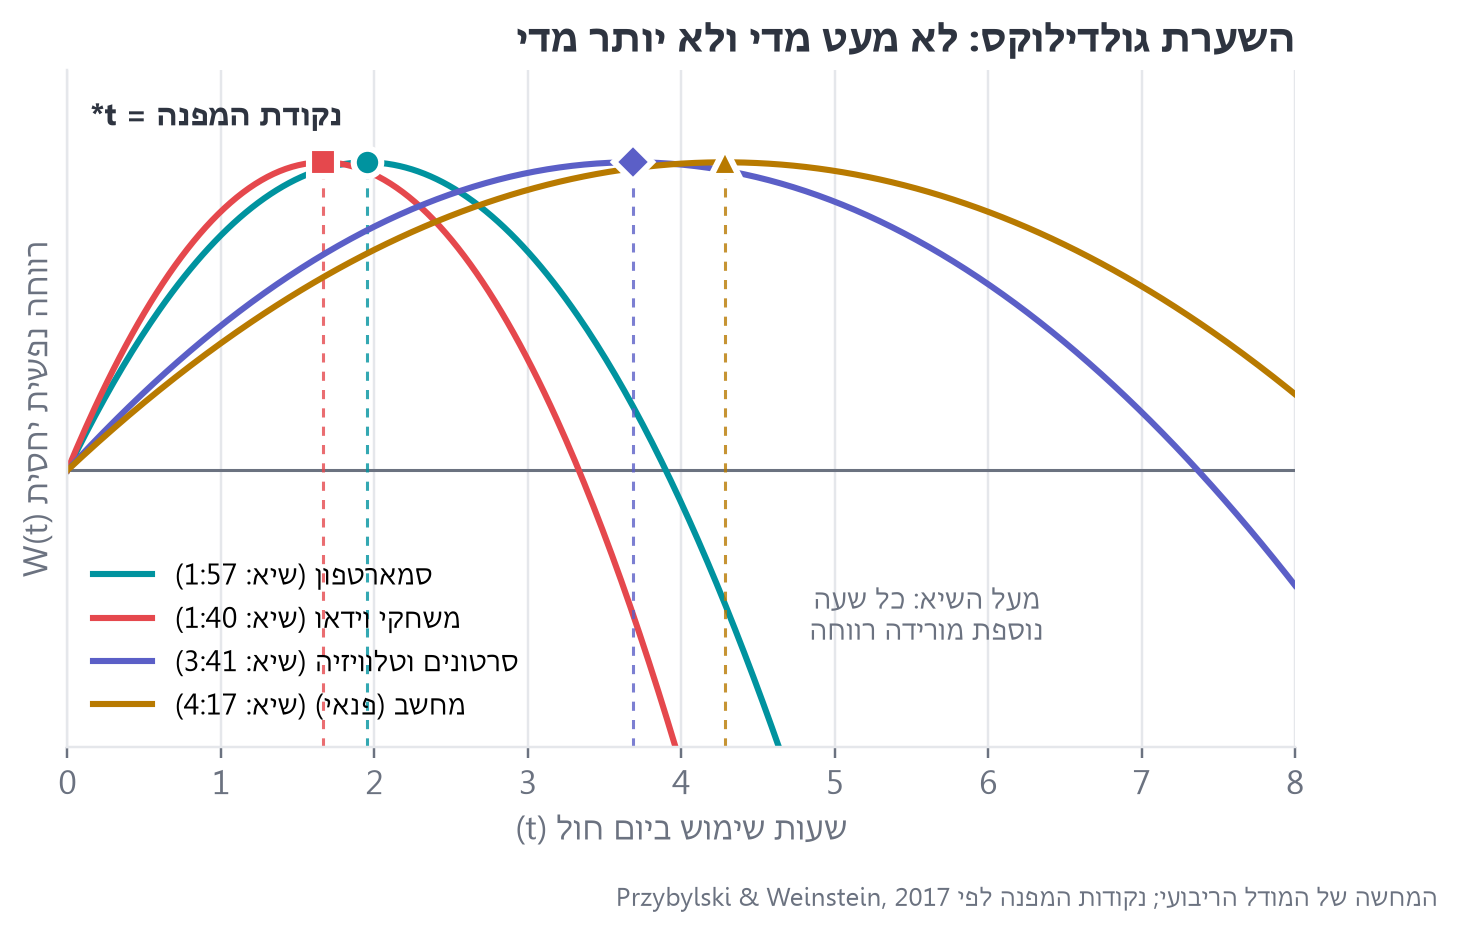
\includegraphics[width=0.92\textwidth]{images/goldilocks.png}
\caption[המחשה של מודל גולדילוקס: נקודת מפנה לכל פעילות]{המחשה של מודל גולדילוקס (משוואה~\ref{eq:goldilocks}): לכל פעילות יש נקודת מפנה $t^{*}$ משלה. נקודות המפנה לימי חול לפי \textcite{przybylski2017}. העקומות בנויות כך שהשיא ייפול על נקודת המפנה, והגובה השווה שלהן הוא נרמול: הן מראות \textbf{איפה} השיא, לא כמה הוא גבוה. האפקט שנמדד בפועל קטן \parencite{orben2019}.}
\label{fig:goldilocks}
\end{figure}


איור~\ref{fig:goldilocks} מציג ארבע עקומות להמחשה, אחת לכל פעילות, וכל אחת מגיעה לשיא בנקודת המפנה שדווחה עבור ימי חול \parencite{przybylski2017}:

\begin{itemize}
  \item \textbf{סמארטפון}: כשעה ו-57 דקות ביום.
  \item \textbf{משחקי וידאו}: כשעה ו-40 דקות ביום (ובסוף השבוע כ-3 שעות ו-35 דקות).
  \item \textbf{צפייה בסרטונים ובטלוויזיה}: כ-3 שעות ו-41 דקות ביום (ובסוף השבוע כ-4 שעות ו-50 דקות).
  \item \textbf{מחשב לשימוש פנאי}: כ-4 שעות ו-17 דקות ביום.
\end{itemize}

במילים פשוטות: בערך שעתיים בסמארטפון ביום חול, ועד כארבע שעות ויותר בצפייה וביישומי מחשב. הסמארטפון, המכשיר הקרוב ביותר לגוף, ומשחקי הווידאו מגיעים לנקודת המפנה מהר ביותר, עוד לפני שתי שעות ביום.

\begin{alertbox}[זהירות: אפקט קטן, קשר ולא סיבה]
שני דברים חשוב לזכור. ראשית, \textbf{האפקט חלש}. גם בשימוש גבוה, ההבדל ברווחה קטן \parencite{przybylski2017}. שנית, זה \textbf{מחקר מתאמי}: הוא מראה ששני דברים הולכים יחד, לא שאחד גורם לשני. ייתכן שמתבגרים שמרגישים רע פונים יותר למסכים, ולא להפך. ניתוח מאוחר יותר של מדגמים גדולים מצא קשר שלילי קטן מאוד בין שימוש בטכנולוגיה לבין רווחת מתבגרים \parencite{orben2019}.
\end{alertbox}

\section{ויכוח אמיתי}

כאן נכנס לתמונה הוויכוח הסוער ביותר בתחום. הפסיכולוג החברתי ג'ונתן הייט טוען שבין 2010 ל-2015 בערך התרחשה \en{the Great Rewiring of Childhood}, "החיווט מחדש הגדול של הילדות": מעבר מילדות שמבוססת על משחק לילדות שמבוססת על טלפון. לדבריו, זה גורם מרכזי במשבר בריאות הנפש של בני נוער \parencite{haidt2024}.

מנגד, איימי אורבן ואנדרו פשיבילסקי מזהירים מהכללות רחבות. לפי הניתוח שלהם, הקשר הממוצע בין טכנולוגיה דיגיטלית לרווחה הוא שלילי, אבל קטן מאוד, ואין להפוך אותו לסיפור של קטסטרופה \parencite{orben2019}.

מי צודק? ייתכן ששניהם, חלקית. ממוצעים קטנים יכולים להסתיר קבוצות שנפגעות מאוד. ומצד שני, בהלה מוסרית יכולה להסיט את תשומת הלב מגורמים אחרים, כמו לחץ בלימודים, מצב כלכלי או בדידות. זה לא ויכוח בין מדע לבורות. זה ויכוח בתוך המדע, והוא עדיין לא הוכרע.

\begin{thinkbox}
אם ההבדל הממוצע קטן, האם זה אומר שאין בעיה? או שמא בעיה קטנה אצל מיליארד אנשים היא, בסופו של דבר, בעיה גדולה מאוד?
\end{thinkbox}

\chapter{הבית החכם והאינטרנט של הדברים}

\begin{epigraph}{}
פעם נעלנו את הדלת כדי שאיש לא יידע מה קורה בפנים. היום הדלת עצמה יודעת, ומדווחת.
\end{epigraph}

\section{הבית שמקשיב}

במשך עשרות אלפי שנים, הבית היה המקום שבו מסתתרים מהעולם. מערה, אוהל, בקתה, דירה. קירות עבים, דלת נעולה, ובפנים פרטיות. ההיסטוריה של האדריכלות היא במידה רבה היסטוריה של הפרדה בין "בפנים" לבין "בחוץ".

הבית החכם מטשטש את הגבול הזה. הנורה נדלקת כשאתם נכנסים. התרמוסטט לומד באיזו שעה אתם חוזרים מהעבודה. הרמקול בסלון מחכה למילת ההפעלה, ובשביל זה הוא צריך להקשיב כל הזמן. המקרר יודע מתי נגמר החלב, והשואב הרובוטי מכיר את מפת הדירה טוב יותר מהאורחים.

כל זה נכנס תחת שם כללי: \textbf{האינטרנט של הדברים} (\en{Internet of Things}, או \en{IoT}). הרעיון פשוט. לא רק אנשים מתחברים לרשת, אלא גם חפצים. והחפצים, בניגוד לאנשים, לא ישנים אף פעם.

\begin{figure}[!htb]\centering
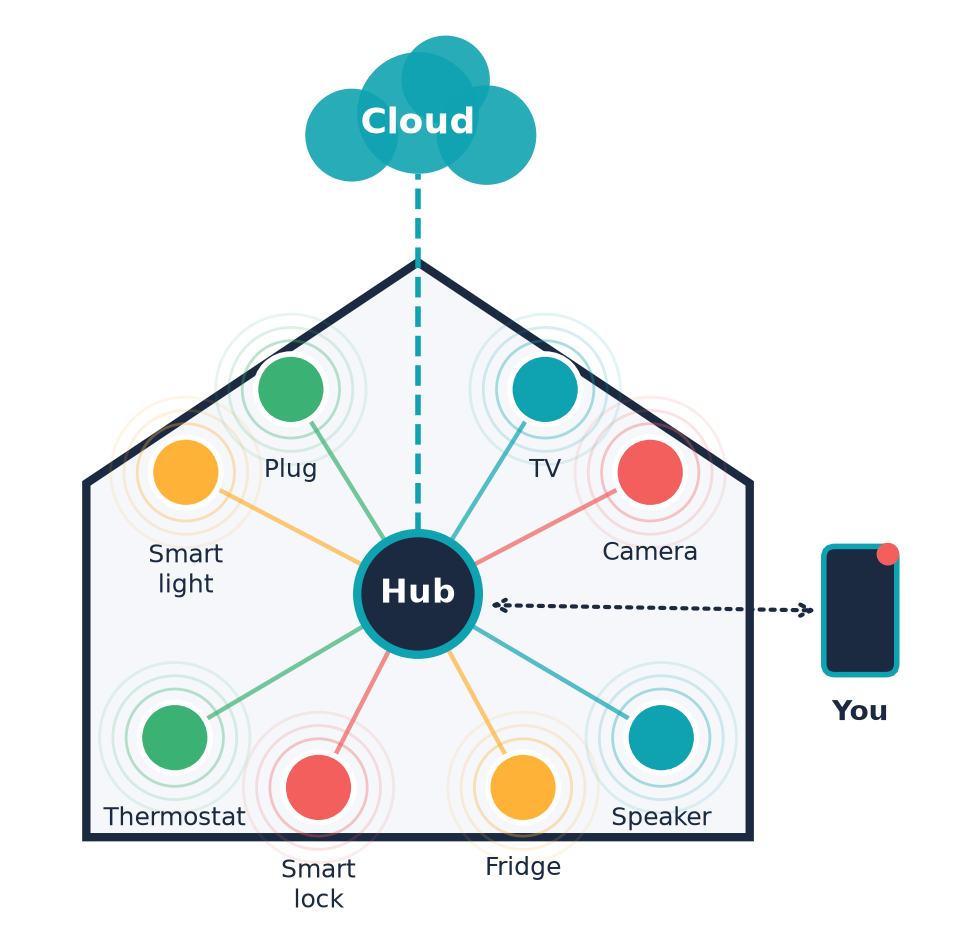
\includegraphics[width=0.85\textwidth]{images/smart_home.png}
\caption[הבית החכם: מכשירים מחוברים לרשת]{הבית החכם: מכשירים יומיומיים שמחוברים לרשת ומתקשרים זה עם זה ועם הענן. האיור נוצר ב-\en{Python}.}\label{fig:smart-home}\end{figure}

איור~\ref{fig:smart-home} ממחיש את הרעיון. כל מכשיר בבית הוא צומת ברשת. כל אחד מהם אוסף מידע קטן ותמים לכאורה: טמפרטורה, תנועה, צריכת חשמל, קול. אבל כשמחברים את כל הנקודות, מתקבלת תמונה מפורטת להפתיע של החיים בתוך הבית.

\section{יותר משמונה-עשר מיליארד חפצים מחוברים}

כמה "דברים" כבר מחוברים? לפי חברת המחקר \en{IoT Analytics}, ב-\num{2024} היו בעולם כ-\num{18.5} מיליארד מכשירים מחוברים. בדוח שפרסמה באוקטובר \num{2025} היא חזתה כ-\num{21.1} מיליארד עד סוף \num{2025} \parencite{iotanalytics2025}. כלומר, \num{18.5} הוא הנתון המדוד האחרון בדוח, ו-\num{21.1} הוא תחזית שפורסמה לפני סוף השנה, לא מדידה. צריך לקרוא את המספר הזה בזהירות. רובם המכריע של המכשירים האלה אינם בבתים: המספר כולל גם חיישנים במפעלים, בחקלאות ובתחבורה. לכן הוא איננו מודד בתים חכמים, ואין טעם להעמיד אותו מול מספר בני האדם המחוברים. מה שהוא כן מראה הוא שהרשת כבר איננה רק רשת של בני אדם.

\begin{factbox}[מכשירים מחוברים בעולם]
\begin{itemize}
  \item 2022: כ-14.4 מיליארד
  \item 2023: כ-16.7 מיליארד
  \item 2024: כ-18.5 מיליארד
  \item 2025: כ-21.1 מיליארד (תחזית מאוקטובר \num{2025})
  \item 2030: כ-39 מיליארד (תחזית מאוקטובר \num{2025})
\end{itemize}
מקור: \textcite{iotanalytics2025}. כל המכשירים המחוברים בעולם, לא רק בבתים.
\end{factbox}

הסדרה הזאת מראה האצה. בין 2022 ל-2024 נוספו כארבעה מיליארד מכשירים בתוך שנתיים. אם תחזית \num{2025}, שפורסמה באוקטובר של אותה שנה, התממשה, הרי שבתוך שלוש שנים בלבד נוספו כשבעה מיליארד מכשירים, ולפי התחזית, עד 2030 המספר יגדל פי שניים ויותר לעומת 2024 \parencite{iotanalytics2025}. אלה תחזיות של חברת מחקר, לא מדידות, והן כוללות את כל המכשירים המחוברים, לא רק את אלה שבבית. הרשת, שהתחילה כקשר בין כמה מחשבים באוניברסיטאות, הופכת למערכת עצבים שעוטפת את כדור הארץ.

\section{נוחות במחיר פרטיות}

למה בכלל להכניס את כל זה הביתה? כי זה נוח, ולעיתים אפילו מציל חיים. חיישן עשן ששולח התראה לטלפון כשאתם רחוקים. מנעול שנפתח לילד ששכח מפתח. מערכת שמזכירה לקשיש ליטול תרופה. מזגן שנכבה כשאיש לא בבית וחוסך חשמל. אין כאן רק שעשועים. יש כאן שירותים אמיתיים.

אבל לכל נוחות יש מחיר, והמחיר כאן הוא מידע. מי שיודע מתי האורות כבים יודע מתי אתם ישנים. מי שיודע מתי הדלת נפתחת יודע מתי הבית ריק. ומי שמקשיב לסלון, גם אם רק לצורך זיהוי מילת הפעלה, נמצא קרוב מאוד לשיחות הפרטיות ביותר שלכם.

זוכרים את מעגל כלכלת הקשב מפרק~\ref{ch:attention}? שושנה זובוף תיארה כיצד החוויה האנושית הופכת לחומר גלם לנתוני התנהגות \parencite{zuboff2019}. הבית החכם מרחיב את המכרה הזה אל המקום האינטימי ביותר שיש. אם הסמארטפון יודע מה אתם עושים בחוץ, הבית החכם יודע מה אתם עושים בפנים.

\begin{alertbox}[שאלות לפני שמחברים מכשיר חדש]
\begin{itemize}
  \item איזה מידע המכשיר אוסף, והאם הוא באמת צריך אותו כדי לעבוד?
  \item לאן המידע נשלח, ולכמה זמן הוא נשמר?
  \item האם אפשר לכבות את המיקרופון או את המצלמה בלחיצה פיזית?
  \item מה יקרה למכשיר, ולמידע, אם החברה שמאחוריו תיסגר או תימכר?
\end{itemize}
\end{alertbox}

\section{מי הבעלים של המטבח שלכם?}

יש כאן גם שאלה עמוקה יותר, שקשורה לבעלות. במשך רוב ההיסטוריה, כשקניתם כיסא, הכיסא היה שלכם. אף אחד לא יכול היה לשנות אותו מרחוק. היום, מכשיר חכם הוא במידה רבה שירות. החברה יכולה לעדכן אותו, לשנות את התנאים, להוסיף פרסומות, או להפסיק לתמוך בו. ייתכן שקניתם את הקופסה, אבל לא את מה שמתרחש בתוכה.

ויש גם צד ביטחוני. כל מכשיר מחובר הוא דלת נוספת אל הרשת הביתית. מצלמה זולה עם סיסמת ברירת מחדל, נורה שלא קיבלה עדכון אבטחה כבר שנים, או צעצוע שמדבר עם הענן, עלולים להפוך לנקודת תורפה. בעולם הישן, פורץ היה צריך לשבור חלון. בעולם החדש, לפעמים מספיק לו שמישהו שכח לשנות סיסמה.

ובכל זאת, אם להסתכל לאחור במבט רחב, נדמה שטכנולוגיות ביתיות חדשות רבות עוררו בהתחלה חשד. החשמל נראה מסוכן, הטלפון נראה פולשני, והטלוויזיה נראתה כמו אורח שלא הולך הביתה. עם הזמן פיתחו החברות האנושיות כללים, תקנים וחוקים שהפכו כל אחת מהטכנולוגיות האלה לבטוחה יותר. סביר להניח שזה יקרה גם עם הבית החכם. השאלה היא כמה מידע נאבד בדרך, עד שהכללים יתעדכנו.

זה לא אומר שצריך לחזור לנרות ולמפתחות ברזל. זה אומר שהשאלה "האם זה נוח?" צריכה לבוא יחד עם שאלה נוספת: "מי עוד נהנה מהנוחות שלי?".

\begin{thinkbox}
דמיינו שכל המידע שנאסף בבית שלכם במשך שנה מודפס בספר אחד. האם הייתם מסכימים שזר יקרא אותו? ואם לא, למה אתם מסכימים שמחשב של זר יקרא אותו?
\end{thinkbox}

\chapter{איזון דיגיטלי: ארגז כלים}

\begin{epigraph}{}
לא צריך לשבור את הכלי. מספיק לזכור מי מחזיק בו.
\end{epigraph}

\section{לא לזרוק את הטלפון לים}

בתחילת המהפכה התעשייתית, באנגליה של המאה ה-19, היו פועלים שפרצו למפעלים וניפצו את מכונות האריגה. הם נודעו בשם "לודיטים", ושמם הפך מאז לכינוי גנאי למי שמתנגד לקדמה. אבל הלודיטים לא שנאו מכונות. הם פחדו ממה שהמכונות עושות לחיים שלהם. ובמובן מסוים, הם שאלו את השאלה הנכונה, גם אם בחרו בתשובה הלא נכונה.

גם אנחנו לא צריכים לנפץ את הטלפונים. רוב האנשים לא ייפרדו מהסמארטפון, ואין סיבה שייפרדו. הוא מחבר אותנו למשפחה רחוקה, מציל אותנו מהליכה לאיבוד, ומאפשר ללמוד כמעט כל דבר. המטרה איננה לחזור למערה. המטרה היא לעבור ממצב שבו המכשיר משתמש בנו למצב שבו אנחנו משתמשים בו.

והמחקר תומך בגישה הזאת. מודל גולדילוקס מפרק~\ref{ch:wellbeing} לא המליץ על אפס מסכים. הוא הצביע על \textbf{מתינות}: שימוש מתון אינו מזיק מטבעו, ורק שימוש מוגזם קשור לירידה ברווחה \parencite{przybylski2017}. במילים אחרות, המטרה היא לא לנצח את הטכנולוגיה, אלא למצוא את הדייסה שהיא "בדיוק כמו שצריך".

\section{מינימליזם דיגיטלי}

קל ניופורט, מדען מחשב, מציע בספרו "מינימליזם דיגיטלי" פילוסופיה פשוטה לכאורה: במקום לשאול "האם לכלי הזה יש תועלת כלשהי?", שאלו "האם הוא משרת את הדברים שהכי חשובים לי?" \parencite{newport2019}. כמעט לכל אפליקציה יש תועלת כלשהי. זו בדיוק הבעיה. אם נאמץ כל כלי שיש בו משהו טוב, לא יישאר לנו זמן לשום דבר אחר.

ניופורט מצביע גם על מחיר שקט שקל לפספס: \textbf{מחסור בבדידות} (\en{solitude deprivation}) \parencite{newport2019}. הכוונה לא לבדידות במובן של עצב, אלא לרגעים שבהם אנחנו לבד עם המחשבות שלנו, בלי קלט מאף אדם אחר. בעבר, רגעים כאלה הגיעו מעצמם: בתור לבנק, באוטובוס, בהליכה הביתה. היום כל רגע ריק מתמלא מיד במסך. ואולי דווקא ברגעים הריקים האלה נולדו פעם רוב הרעיונות הטובים.

\begin{tipbox}[טיפ: התחילו בערכים, לא בכלים]
לפני שאתם מוחקים אפליקציות, כתבו שלושה דברים שהכי חשובים לכם בחיים. אחר כך עברו על המסך הראשי בטלפון ושאלו על כל אפליקציה: האם היא מקרבת אותי לאחד מהם?
\end{tipbox}

\section{גבולות לדור הבא}

ג'ונתן הייט, שהכרנו בפרק~\ref{ch:wellbeing}, טוען שהמעבר מילדות מבוססת משחק לילדות מבוססת טלפון הוא גורם מרכזי במשבר בריאות הנפש של בני נוער \parencite{haidt2024}. אחד הרעיונות החשובים שעולים מהדיון הזה הוא שהבעיה איננה רק אישית אלא \textbf{קולקטיבית}. הורה אחד שמחליט לדחות את הסמארטפון של הילד שלו מרגיש שהוא מבודד אותו מחבריו. אבל כשקבוצת הורים, כיתה או בית ספר מחליטים יחד, הלחץ החברתי מתפוגג.

כדאי לזכור שהטענות של הייט שנויות במחלוקת, וחוקרים כמו אורבן ופשיבילסקי מזהירים מהכללות רחבות על סמך אפקטים קטנים \parencite{orben2019}. אבל גם מי שלא משוכנע לגמרי יכול להסכים על עיקרון אחד: החלטות על ילדות צריכות להתקבל בכוונה, ולא כברירת מחדל של אפליקציה.

\begin{alertbox}[בלי מוסר ובלי אשמה]
אם אתם מרגישים שאתם "מכורים", זכרו שמולכם עומדות מערכות שתוכננו בקפידה כדי להחזיק את תשומת הלב שלכם. זה לא כישלון מוסרי. זו מערכה לא הוגנת. המטרה היא לשנות את הסביבה, לא להלקות את עצמכם.
\end{alertbox}

\section{ארגז הכלים}

הנה כמה כלים מעשיים. אין צורך לאמץ את כולם. בחרו שניים או שלושה, נסו אותם שבועיים, ובדקו מה השתנה.

\begin{tipbox}[טיפ 1: שנו את ברירת המחדל]
כבו את כל ההתראות, חוץ מאלה שמגיעות מבני אדם אמיתיים שחשובים לכם. זכרו את מעגל כלכלת הקשב: הטריגר הוא השלב הראשון. בלי טריגר, המעגל מתחיל הרבה פחות פעמים.
\end{tipbox}

\begin{tipbox}[טיפ 2: הרחיקו את המכשיר מהמיטה]
קנו שעון מעורר פשוט, והטעינו את הטלפון מחוץ לחדר השינה. כך הדבר הראשון והאחרון שתראו ביום לא יהיה מסך.
\end{tipbox}

\begin{tipbox}[טיפ 3: הפכו את הגלילה לקשה יותר]
העבירו את האפליקציות הממכרות למסך השני, לתיקייה, או התנתקו מהן אחרי כל שימוש. כל שנייה של מאמץ נותנת למוח הזדמנות לשאול: אני באמת רוצה את זה?
\end{tipbox}

\begin{tipbox}[טיפ 4: החזירו את השעמום]
הקדישו כל יום כמה דקות לבדידות אמיתית: הליכה בלי אוזניות, המתנה בתור בלי מסך. השעמום הוא לא אויב. הוא חדר ההמתנה של היצירתיות.
\end{tipbox}

ולבסוף, רשימת תיוג לשבוע הקרוב:

\begin{checklist}
  \item כיביתי התראות שאינן מגיעות מבני אדם.
  \item הטלפון נטען הלילה מחוץ לחדר השינה.
  \item אכלתי לפחות ארוחה אחת ביום בלי מסך על השולחן.
  \item בדקתי את נתוני זמן המסך שלי, בלי לשפוט, רק כדי לדעת.
  \item מחקתי או הסתרתי אפליקציה אחת שאינה משרתת את הערכים שלי.
  \item יצאתי להליכה של רבע שעה בלי אוזניות.
  \item דיברתי עם המשפחה או עם החברים על כללים משותפים לשימוש במסכים.
\end{checklist}

\begin{thinkbox}
דמיינו שבעוד עשר שנים אתם מסתכלים אחורה על השבוע הזה. על אילו דקות מול המסך תשמחו? ועל אילו תצטערו?
\end{thinkbox}

\chapter{סיכום ומבט לעתיד}

\begin{epigraph}{}
השאלה איננה מה הטכנולוגיה תעשה לנו. השאלה היא מה נבחר לעשות איתה.
\end{epigraph}

\section{מה למדנו}

התחלנו את המסע ביד שנשלחת אל הטלפון עוד לפני שהעיניים נפתחות. בדרך עברנו מהמברק של 1844 אל הסמארטפון של 2007, וראינו איך המידע, שבמשך רוב ההיסטוריה נע במהירות של רגליים, התחיל לנוע במהירות האור.

\begin{sloppypar}
כמה מספרים מסכמים את התמונה. כ-5.87 מיליארד בני אדם השתמשו באינטרנט ב-2024 \parencite{itu2026data}, ובישראל כ-91.1\% מהאוכלוסייה מחוברים \parencite{kemp2025israel}. משתמש טיפוסי מבלה ברשת כ-6 שעות ו-40 דקות ביום \parencite{kemp2024}. בבתים, במפעלים וברחובות פועלים כ-18.5 מיליארד מכשירים מחוברים \parencite{iotanalytics2025}. והמחקר מרמז שבסמארטפון, נקודת המפנה של הרווחה בימי חול מגיעה כבר אחרי כשעתיים ביום \parencite{przybylski2017}.
\end{sloppypar}

אבל הלקח החשוב ביותר איננו מספר. הוא מנגנון. ראינו שהקשב הפך למשאב הנדיר של התקופה \parencite{simon1971}, ושסביבו נבנתה כלכלה שלמה, שהופכת כל גלילה לנתון וכל נתון לתחזית \parencite{zuboff2019}. ראינו שהקשר בין מסכים לרווחה אמיתי, אבל קטן ומורכב, ושהמדענים עצמם עדיין מתווכחים עליו \parencite{orben2019,haidt2024}. וראינו שהאיזון אפשרי, לא דרך התנזרות, אלא דרך בחירה מודעת.

\section{מבט קדימה: המכונה שמדברת}

פגשנו את \en{ChatGPT} כבר בפרק השני: מוצר שהושק בסוף 2022 בלי תרועות, כניסוי \parencite{openai2022}. בדיעבד, זה עשוי להתברר כרגע היסטורי בסדר גודל של המברק.

עד עכשיו, כל טכנולוגיות התקשורת שתיארנו בספר הזה העבירו מילים שבני אדם כתבו. המברק, הטלפון, הרדיו, האינטרנט והרשתות החברתיות היו כולם צינורות. הבינה המלאכותית היא משהו אחר. היא לא רק מעבירה את הסיפורים שלנו. היא מספרת סיפורים משלה.

מה זה יעשה לכלכלת הקשב? אם עד היום אלגוריתמים \textbf{בחרו} איזה תוכן להראות לנו, בקרוב הם עשויים \textbf{ליצור} אותו, במיוחד עבורנו, בכל רגע. מצד אחד, זו הבטחה מרגשת: מורה פרטי לכל ילד, עוזר אישי לכל אדם, ידע שזמין בכל שפה. מצד שני, מערכת שיודעת לשוחח איתנו בחום ובסבלנות אינסופית עלולה להיות מושכת עוד יותר מכל פיד.

כל הכלים שפגשנו בספר הזה רלוונטיים גם כאן. מודל גולדילוקס מזכיר לנו לשאול לא רק "האם", אלא "כמה ומאיזה סוג". המעגל של כלכלת הקשב מזכיר לנו לשאול מי משלם ומי מרוויח. וארגז הכלים מזכיר לנו שגם מול מערכות חכמות מאוד, יש לנו עדיין שליטה על ברירות המחדל של החיים שלנו.

\begin{alertbox}[השאלות החדשות]
\begin{itemize}
  \item כשמכונה כותבת, איך נדע מה אמיתי?
  \item כשעוזר דיגיטלי מכיר אותנו טוב יותר מחברים, למי נפנה ברגע של משבר?
  \item ומי יקבע מה הבינה המלאכותית תגיד לנו, ולמה?
\end{itemize}
\end{alertbox}

\section{שאלה אחרונה}

בני האדם תמיד היו יצורים מחוברים. הציידים-לקטים היו תלויים בשבט שלהם כדי לשרוד. הקשרים האלה הם שהפכו קוף חסר חשיבות מאפריקה לשליט כדור הארץ. במובן הזה, הסמארטפון לא המציא שום דבר חדש. הוא רק לקח את הצורך העתיק ביותר שלנו, הצורך להיות חלק ממשהו, והגביר אותו לעוצמה שלא הכרנו מעולם.

השאלה איננה אם להיות מחוברים. זה כבר הוחלט, ובצדק. השאלה היא למה אנחנו מתחברים, ומה אנחנו מוכנים לתת בתמורה.

\begin{thinkbox}[השאלה שנשארת איתכם]
אם הקשב שלכם הוא המשאב היקר ביותר שיש לכם, ואם יש בעולם מערכות חכמות מאוד שמתחרות עליו בכל רגע, את מי אתם בוחרים לשים במרכז שלו?
\end{thinkbox}

אולי כדאי לחשוב על זה רגע. ואולי, רק הפעם, לעשות את זה בלי הטלפון ביד.


% ---------- ביבליוגרפיה ----------
\chapter*{רשימת מקורות}
\addcontentsline{toc}{chapter}{רשימת מקורות}
\markboth{רשימת מקורות}{}
\begin{english}
\printbibliography[heading=none]
\end{english}

\end{document}
